\newcommand{\basedir}{fablab-document}
\documentclass{\basedir/fablab-document}

\usepackage{minitoc} % Inhaltsübersicht je Section
% \usepackage{fancybox} %ovale Boxen für Knöpfe - nicht mehr benötigt
\usepackage{amssymb} % Symbole für Knöpfe
% \usepackage{subfigure,caption}
\usepackage{eurosym}
\usepackage{tabularx} % Tabellen mit bestimmtem Breitenverhältnis der Spalten
\usepackage{wrapfig} % Textumlauf um Bilder
\usepackage{todonotes}
\usepackage{framed}
\usepackage{xargs}
\usepackage{framed}
\usepackage{multirow}

\renewenvironmentx{leftbar}[3][2=0.5pt, 3=5pt]{\def\FrameCommand{\vrule width #2 \hspace{#3}}\MakeFramed {\advance\hsize-\width \FrameRestore}{\tiny#1\\}} {\endMakeFramed}

\renewcommand{\texteuro}{\euro}

\linespread{1.2}

\date{Februar 2016}
\author{FAU FabLab} % Siehe github commits für Authoren
\title{Einweisung Oberfräse}

\begin{document}
 % Hinweise an Package minitoc, doch bitte irgendwas zu generieren - wird für späteres \secttoc benötigt
\dosecttoc
\faketableofcontents
\mtcsettitle{secttoc}{Arbeitsschritte}
\mtcsettitlefont{secttoc}{\large \sffamily \bfseries}
\mtcsetfont{secttoc}{subsection}{\sffamily}
% \mtcset
% hier geht das eigentliche Dokument los

%\color{red}
%\hrule
%\begin{center}
%\large{Achtung! Einweisung ist noch in Arbeit!}
%\vspace{0.1cm}
%\end{center}
%\hrule
%\color{black}

\section{Technische Daten}
\begin{tabular}{r|l}
Hersteller & Festool \\
Produktname & Oberfräse OF 1010 EBQ \\
Leistung & $1010\,\mathrm{Watt}$ \\
Drezahlbereich & $10.000 - 24.000\,\mathrm{min}^{-1}$ \\
Fräserdurchmesser & max. $35\,\mathrm{mm}$ \\
\multirow{2}{*}{Fräserschaftdurchmesser} & $8\,\mathrm{mm}$ (Spannzange vorhanden)\\
                        & $6,0$ und $6,35\,\mathrm{mm}$ (Spannzangen nicht vorhanden) \\
\end{tabular}


\section[Allgemeine Sicherheitshinweise]{Allgemeine Sicherheitshinweise}
\begin{itemize}
\item {\color{red} Vor dem eigenständigen Gebrauch muss eine Einweisung durch einen Betreuer erfolgt und unterschrieben worden sein. Zum Erlangen der Nutzungsberechtigung muss die sichere und schonende Handhabung der Maschine für Nutzer, Werkzeug und Umgebung gezeigt worden sein.}
\item Werkstück immer gut festspannen, nie in der Hand oder von Dritten halten lassen
\item Maschine stets an beiden Griffen (1.17 und 1.15) halten und führen
\item Immer im Gegenlauf fräsen, entsprechend des Pfeils auf dem Frästisch (rot markiert, 1.11)
\item Maschine zuerst einschalten und erst danach ins Werkstück eintauchen
\item Vor Werkzeugwechsel Maschine vom Stromnetz trennen -- Stecker ziehen
\item Werkzeug fest einspannen -- dazu Schlüssel aus der Maschinenkiste oder 19mm Maulschlüssel verwenden
\item Keine defekten, rissigen, verbogenen oder stumpfen Werkzeuge verwenden
\item Unbedingt mit aktivem Staubsauger fräsen
\item Netzkabel aus dem Eingriffsbereich des Fräsers halten
\item Die Gefahr einer unbeabsichtigten Betätigung der Einschaltsperre (1.1) und ``Dauer-Ein''-Stellung beachten und sich damit vertraut machen
\item Nach dem Fräsen Maschine gründlichst reinigen und aussaugen. Zum ausblasen mit Druckluft, Maschine aus dem Fenster halten
\item Im Arbeitsbereich dürfen sich keine Unbeteiligten befinden
\item Wenn möglich, draußen benutzen um den Staub der sich im Lab absetzt zu reduzieren
\item Bei Fräsern größer 16mm dürfen nur MAN-Fräser für manuellen Vorschub genutzt werden
\item Die maximale Drehzahl des Fräsers darf nicht überschritten werden
\end{itemize}


\section{Persönliche Schutzausrüstung}
\begin{itemize}
\item Gehörschutz -- hängt an der Fräse, links neben der Werkbank
\item Schutzbrille, unerlässlich bei Bearbeitung von Alu, Faserwerkstoffen und Gipskarton -- hängen hinter der Werkbank und hinter dem Chemiearbeitsbereich an der Wand
\item Bei Hartholz ist der Festool Staubsauger mit Staubklasse M oder besser zu nutzen. Staubmasken befinden sich bei Bedarf in Schublade W9
\item Schutzhandschuhe beim Bearbeiten rauer Materialien und beim Werkzeugwechsel -- liegen in der Schutzausrüstungsschublade W9
\item Offene lange Haare sind zurückzubinden. Es besteht die Gefahr des Einzugs in rotierende Maschinenelemente.

\end{itemize}

\begin{figure}[h!]
    \centering
    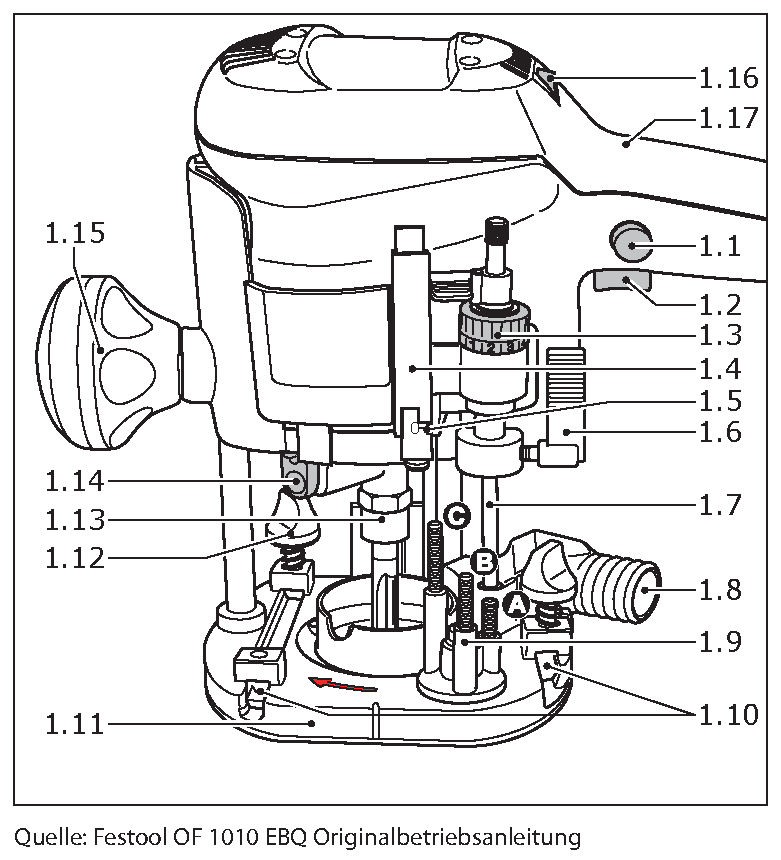
\includegraphics[width=0.8\textwidth]{bilder/oberfraese-sketch}
    \caption{Festool Oberfräse OF 1010 EBQ}
    \label{fig:sketch}
\end{figure}

\section{Bestimmungsgemäße Verwendung}
Die Oberfräse ist zur Bearbeitung von Kanten, zum Versäubern und auch zur kreativen Gestaltung (z.b. Einfräsen von Schrift oder Löchern in Plattenmaterial). Es ist wichtig, die folgenden Anweisungen genau zu beachten, damit die Oberfräse nicht zu Gesundheitsschäden führt oder beschädigt wird.\\
Es dürfen mit der Maschine Holz, Kunststoff und Aluminium bearbeitet werden, dabei immer auf die richtige Fräserauswahl achten. Bei der Verwendung der Maschine sollte nur der Festool-Staubsauger verwendet werden, da sonst sehr viel Staub und Dreck entsteht. Dabei ist zu beachten, dass die Oberfräse an einer Steckdose des Festool-Saugers angeschlossen wird und der Sauger selbst auf \enquote{AUTO} sowie voller Saugleistung steht. Bei Holz kann sich der Einlass der Absaugung (1.8) an der Oberfräse durch Holzsplitter zusetzen. Bei geringem Absaugeffekt ist die Arbeit zu unterbrechen und die Problemstelle zu finden.\\
\textbf{WICHTIG: Die Oberfräse darf ausschließlich von eingewiesene Personen verwendet werden.}


\subsection{Aluminiumbearbeitung}
Bei der Bearbeitung von Aluminium sind aus Sicherheitsgründen folgende besonderen Maßnahmen einzuhalten:
\begin{itemize}
\item Maschine nur mit dem Festool-Absaugwagen verwenden, da heiße Späne abgesaugt werden.
\item Maschine nach der Arbeit von Staubablagerungen im Motorgehäuse reinigen, um langfristig Kurzschlüsse zu vermeiden.
\item Nur geeignete Fräser verwenden (NICHT die Festool Fräser).
\item Es entstehen große Kräfte, daher nur kleinere Fräser nutzen.
\end{itemize}


\section{Inbetriebnahme}
Maschine vor dem Anschließen und entfernen des Stromkabels stets ausschalten! Dazu Ein-/Ausschalter (1.2) drücken und kontrollieren, dass die Einschaltsperre (1.1) herausspringt.

\section{Einstellungen}
\subsection{Funktionen der Maschine}
\begin{itemize}
%\item Sanftanlauf: Der elektronisch geregelte Sanftanlauf sorgt für ruckfreien Anlauf des Elektrowerkzeugs.
%\item Konstante Drehzahl: Die Motordrehzahl wird elektronisch konstant gehalten. Dadurch wird auch bei Belastung eine gleichbleibende Schnittgeschwindigkeit erreicht.
% Ist das wirklich eine Relevantefunktion, die zu beachten ist. Klar ist das schön, aber darauf achten muss man doch nicht. (jh)
\item Drehzahlregelung: Die Drehzahl lässt sich mit dem Stellrad (1.16) stufenlos einstellen. Dadurch kann die Schnittgeschwindigkeit der jeweiligen Oberfläche optimal angepasst werden
\item Temperatursicherung: Bei zu hoher Motortemperatur werden Stromzufuhr und Drehzahl reduziert. Die Maschine läuft nur noch mit verringerter Leistung, um eine rasche Abkühlung durch die Motorlüftung zu ermöglichen. Wenn die Übertemperatur andauert, schaltet die Maschine nach ca. 40 sec komplett ab. Erst nach Abkühlung des Motors ist ein erneutes Einschalten möglich.
\item Strombegrenzung: Die Strombegrenzung verhindert bei extremer Überlastung eine zu hohe Stromaufnahme. Dies kann zu einer Verringerung der Motordrehzahl führen. Nach Entlastung läuft der Motor sofort wieder an.
\item Bremse: Die \textit{OF 1010 EBQ} besitzt eine elektronische Bremse. Nach dem Ausschalten wird der Fräser in ca. 2 Sekunden elektronisch zum Stillstand abgebremst.
\end{itemize}

\subsubsection{Fräser wechseln}
\begin{leftbar}{Aus Festool OF 1010 EBQ Handbuch, Abschnitt 5.2 (Anmerkungen in Abschnitt~\ref{quellen} beachten)}
Für den Werkzeugwechsel können Sie die Maschine auf den Kopf stellen.
\begin{description}
    \item[a)] Werkzeugeinsetzen
        \begin{itemize}
            \item Stecken Sie das Fräswerkzeug so weit wie möglich, zumindest jedoch bis zur Markierung (\underline{V}) am Fräserschaft, in die geöffnete Spannzange.
            \item Verdrehen Sie die Spindel so weit, bis der Spindelstopp (1.14) beim Drücken einrastet und die Spindel arretiert.
            \item Ziehen Sie die Mutter (1.13) mit einem Gabelschlüssel SW 19 fest.
        \end{itemize}
    \item[b)] Werkzeugentnehmen
        \begin{itemize}
            \item Verdrehen Sie die Spindel so weit, bis der Spindelstopp (1.14) beim Drücken einrastet und die Spindel arretiert.
            \item Lösen Sie die Mutter (1.13) mit einem Gabelschlüssel SW 19 so weit, bis Sie einen Widerstand spüren. Überwinden Sie diesen Widerstand durch Weiterdrehen des Gabelschlüssels.
            \item Entnehmen Sie den Fräser.
        \end{itemize}
\end{description}
\end{leftbar}

\subsection{Frästiefe einstellen}
\begin{leftbar}{Aus Festool OF 1010 EBQ Handbuch, Abschnitt 5.4 (Anmerkungen in Abschnitt~\ref{quellen} beachten)}
Das Einstellen der Frästiefe erfolgt in drei Schritten:
\begin{description}
\item[a)] Nullpunkt einstellen
\begin{itemize}
    \item Öffnen Sie den Spannhebel (1.6), so dass der Tiefenanschlag (1.7) frei beweglich ist.
    \item Stellen Sie die Oberfräse mit dem Frästisch (1.11) auf eine ebene Unterlage. Öffnen Sie den Drehknopf (1.15) und drücken Sie die Maschine so weit nach unten bis der Fräser auf der Unterlage aufsitzt.
    \item Klemmen Sie die Maschine durch Schließen des Drehknopfs (1.15) in dieser Stellung fest.
    \item Drücken Sie den Tiefenanschlag gegen einen der drei Festanschläge des drehbaren Revol- veranschlages (1.9).
Mit einem Schraubendreher können Sie jeden Festanschlag individuell in seiner Höhe einstellen:
Festanschlag
A B C
min. Höhe/max. Höhe
38 mm/44 mm 44 mm/54 mm 54 mm/67 mm
    \item Schieben Sie den Zeiger (1.4) nach unten, so dass er auf der Skala (1.5) 0 mm zeigt.
\end{itemize}
\item[b)] Frästiefevorgeben
Die gewünschte Frästiefe lässt sich entweder mit der Tiefenschnellverstellung oder mit der Tiefen- feineinstellung vorgeben.
\begin{description}
    \item[Tiefen-Schnellverstellung] Ziehen Sie den Tiefenanschlag (1.7) so weit nach oben, bis der Zeiger die gewünschte Frästiefe anzeigt. Klemmen Sie den Tiefenanschlag mit dem Spannhebel (1.6) in dieser Stellung fest.
     \item[Tiefen-Feineinstellung] Klemmen Sie den Tiefenanschlag mit dem Spannhebel (1.6) fest. Stel- len Sie die gewünschte Frästiefe durch Drehen des Stellrades (1.3) ein. Wenn Sie das Stellrad um einen Markierungsstrich verdrehen, ändert sich die Frästiefe um 0,1 mm. Eine vollständige Umdrehung ergibt 1 mm. Der maximale Verstellbereich des Stellrades beträgt 8 mm.
\end{description}
\item[c)] Frästiefe zustellen
\begin{itemize}
    \item Öffnen Sie den Drehknopf (1.15) und drücken Sie die Maschine so weit nach unten, bis der Tiefenanschlag den Festanschlag berührt.
    \item Klemmen Sie die Maschine durch Schließen des Drehknopfs (1.15) in dieser Stellung fest.
\end{itemize}
\end{description}
\end{leftbar}

\subsection{Drehzahl wählen}
über das Stellrad 1.16 wird die Drehzahl gewählt, diese hängt vom Material des Werkstücks und dem Fräser ab. Siehe Abbildung~\ref{fig:drehzahl} für Hersteller Empfehlungen
\begin{figure}[h!]
    \centering
    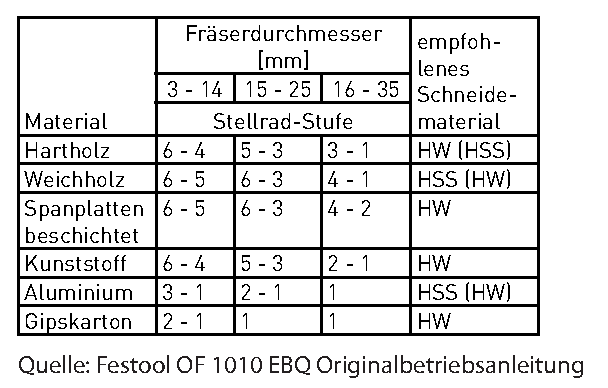
\includegraphics{bilder/drehzahltabelle}
    \caption{Drehzahltabelle}
    \label{fig:drehzahl}
\end{figure}

\section{Arbeiten mit der Maschine}
Beim Arbeiten mit der Maschine ist das Werkstück stets festzuspannen und gegen Verrutschen zu sichern. Die Maschine muss mit beiden Händen gehalten werden. Bei Arbeiten, die gefährliche Stäube erzeugen, ist der Staubsauger auf ``Vollgas'' einzustellen. Hierzu zählt auch Hartholz!

Tipps zum Festspannen:
\begin{itemize}
    \item Sehr kleine Stücke, wo Schraubzwingen das arbeiten mit der Fräse behindern, im Schraubstock so einspannen, dass das Werkstück knapp über die Backen hinausragt. Dabei ist darauf zu achten, dass der Fräser keinesfalls die Backen berührt.
    \item Fräsertiefe beachten, z.B. ragen die Abrundfräser meist nicht auf der Unterseite des Werkstücks heraus, was es erlaubt das Werkstück auf der Werkbank Oberfläche zu platzieren.
\end{itemize}

Immer im Gegenlauf fräsen. Der Fräser dreht bei Draufsicht rechtsherum (siehe Abbildung~\ref{gleichlauf-gegenlauf}), wie auch auf der Grundplatte durch einen Pfeil eingezeichnet. Wenn man also die Fräse von rechts an ein Werkstück heranführt, dann muss zum Bediener hin gefräst werden. Wenn man von rechts an ein Werkstück herangeht, dann von einem weg fräsen. Die Fräse wird so immer einen leichten Gegendruck bieten, den man durch drücken bzw. ziehen ausgleichen muss. Sollte man dies nicht beachten wird die Fräse sich unkontrolliert schnell am Werkstück entlang bewegen, was eine Verletzungsgefahr darstellt und zu sehr schlechten Schnittkanten führt. Zum einfräsen in eine Materialoberfläche empfiehlt es sich zirkular in Drehrichtung des Fräsers einzutauchen.

\begin{figure}[h!]
\centering
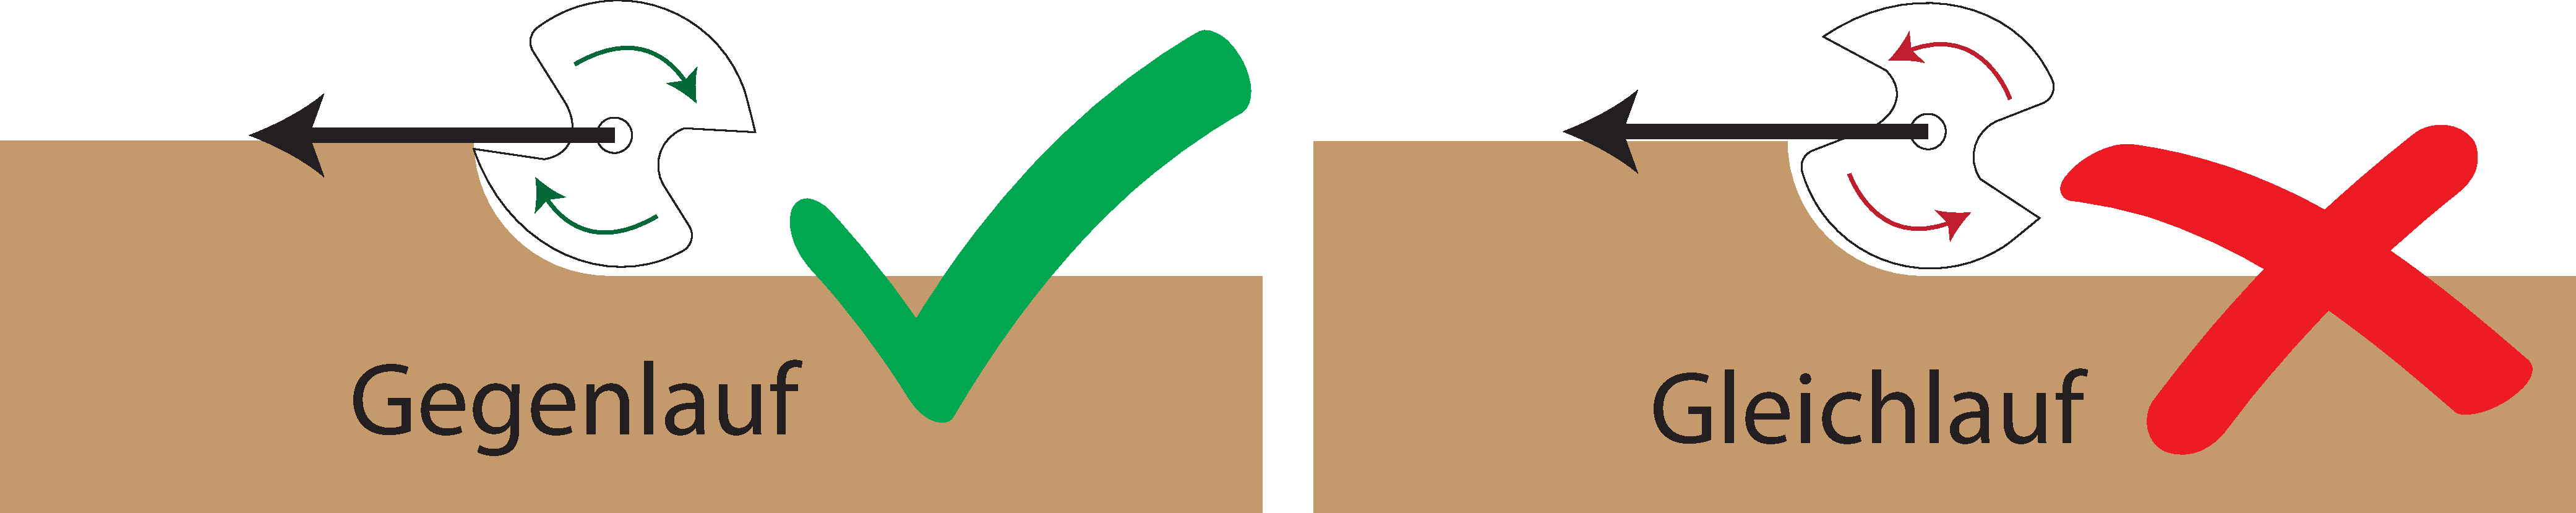
\includegraphics[width=\textwidth]{bilder/gleichlauf-gegenlauf}
\caption{Gegenlauf- und Gleichlauffräsen}
\label{gleichlauf-gegenlauf}
\end{figure}

Tipps für gute Ergebnisse bei Holz:
\begin{itemize}
    \item Rechtwinklig zur Faserstruktur Vorschub leisten. Dies verhindert das Splittern des Holzes entlang der Maserung.
    \item Für den Außengebrauch steht ein Festtool Arbeitstisch zum ausklappen bereit. Wende dich dafür an einen Betreuer.
    \item Die Tiefeneinstellungsskala an der Maschine ist bei Fräsern mit Anschlagring nicht gültig. 
\end{itemize}

Weiteres ist in der Anleitung, ab Seite 9, zu finden.

\section{Arbeiten mit Anschlag und Führung}
\begin{figure}[h!]
    \centering
    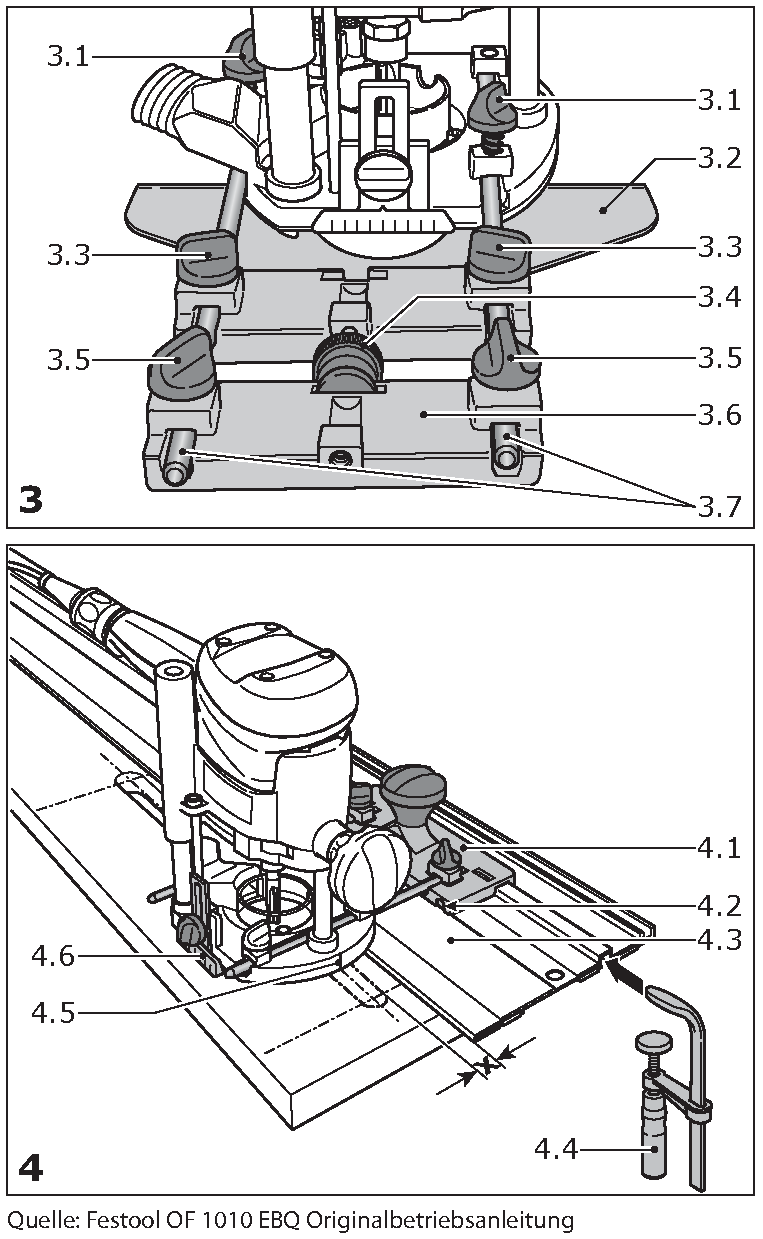
\includegraphics{bilder/fuehrung-sketch}
    \caption{Verwendung von Anschlägen und Führungen}
    \label{fig:drehzahl}
\end{figure}

\begin{leftbar}{Aus Festool OF 1010 EBQ Handbuch, Abschnitte 6.3 und 6.5 (Anmerkungen in Abschnitt~\ref{quellen} beachten)}
\textbf{Fräsen mit Seitenanschlag:}
Für parallel zur Werkstückkante verlaufende
Arbeiten kann der mitgelieferte Seitenanschlag
(3.2) eingesetzt werden (bei ``Modul 5A'' nicht im
Lieferumfang):

\begin{itemize}
    \item Klemmen Sie die beiden Führungsstangen (3.7)
mit den beiden Drehknöpfen (3.3) am Seitenanschlag
fest.
    \item Führen Sie die Führungsstangen bis zum gewünschten
Maß in die Nuten (1.10) des Frästisches
ein und klemmen Sie die Führungsstangen
mit dem Drehknopf (3.1) fest.
\end{itemize}
Schneller und genauer lässt sich dieser Abstand
mit der als Zubehör erhältlichen Feineinstellung
(3.6) justieren:
\begin{itemize}
    \item Drehen Sie die Justierschraube (3.4) in das
Kunststoffteil des Seitenanschlags,
    \item klemmen Sie die Führungsstangen mit den
Drehknöpfen (3.5) an der Feineinstellung fest,
    \item öffnen Sie die Drehknöpfe (3.3) am Seitenanschlag,
    \item stellen Sie den gewünschten Abstand mit der
Justierschraube ein und drehen Sie die Drehköpfe
wieder zu.
\end{itemize}

\textbf{Fräsen mit Anschlag, Führungssystem und Zirkel:}
Das als Zubehör erhältliche Führungssystem
erleichtert das Fräsen gerader Nuten.
\begin{itemize}
    \item Befestigen Sie den Führungsanschlag (4.1) mit
den Führungsstangen (3.7) des Seitenanschlages
am Frästisch.
    \item Befestigen Sie die Führungsschiene (4.3) mit
Schraubzwingen (4.4) am Werkstück. Achten
Sie darauf, dass ein Sicherheitsabstand X (Bild
4) von 5 mm zwischen der Vorderkante der
Führungsschiene und dem Fräser, bzw. der Nut,
besteht.
    \item Setzen Sie den Führungsanschlag, wie in Bild
4 dargestellt, auf die Führungsschiene. Um ein
spielfreies Führen des Fräsanschlages sicherzustellen,
können Sie mit einem Schraubendreher
durch die beiden seitlichen Öffnungen (4.2)
zwei Führungsbacken einstellen.
    \item Schrauben Sie die höhenverstellbare Abstützung
(4.6) so an der Gewindebohrung (6.6) des
Frästisches fest, dass die Unterseite des Frästisches
parallel zur Werkstückoberfläche ist.
\end{itemize}
Um nach Anriss arbeiten zu können, zeigen Ihnen
die Markierung am Frästisch (4.5) und die Skala
an der Abstützung (4.6) die Mittelachse des Fräsers
an.

\textbf{Fräsen mit Stangenzirkel SZ-OF 1000:}
Mit dem als Zubehör erhältlichen Stangenzirkel
SZ-OF 1000 können runde Teile und Kreisausschnitte
mit einem Durchmesser zwischen 153
und 760 mm hergestellt werden.
\begin{itemize}
    \item Schieben Sie den Stangenzirkel so weit in die
vordere Nut des Frästisches, bis der gewünschte
Radius eingestellt ist.
    \item Arretieren Sie den Stangenzirkel mit dem Drehknopf
(1.12).
\end{itemize}
Anwendungstipp:
Soll die Einkerbung durch die Zirkelspitze auf dem
Werkstück vermieden werden, kann mit doppelseitigem
Klebeband ein dünnes Holzbrettchen auf
dem Mittelpunkt befestigt werden.
\end{leftbar}

%\newpage
\section{Quellen und Rechte}
\label{quellen}
Alle Rechte an Grafiken, Tabellen und Textabschnitte, welche aus der Festool Originalbetriebsanleitung übernommen wurden liegen bei Festool. Die \glqq Originalbetriebsanleitung\grqq liegt der Maschine bei und ist online auf \url{www.festool.com} zu finden. Festool hat dieses Dokument weder gelesen, noch auf Vollständigkeit oder Richtigkeit geprüft und übernimmt keine Haftung.
%\begin{itemize}
%\item Festool \glqq Originalbetriebsanleitung\grqq TS 55 REBQ unter 
%\url{http://www.etracker.de/lnkcnt.php?et=6hsNGE&url=https\%3a\%2f\%2fassets.festool.com\%2fmedia\%2f706758_002_ts55rebq.zip&lnkname=Bedienungsanleitung+TS+55}
%\end{itemize}

\end{document}
